\documentclass[14pt,t]{beamer} % beamer - typ/šablona prezentace

\usepackage[czech]{babel} % nastavuje české popisky např. u obsahu, referencí, tabulek, obázků 
\usepackage[utf8]{inputenc} % použito UTF8 kvůli češtině (zvládá prakticky všechny jazyky na světě)
\usepackage[T1]{fontenc}

\usepackage{lmodern}
%\usepackage{datetime}
\usepackage{amssymb} % podpůrná knihovna pro matematické symboly
\usepackage{enumerate} % umožňuje širší možnosti nastavení enumerate

\usepackage{graphicx} % vkládání obrázků
\usepackage{hologo} % logo BibTeX

\usepackage{multicol} % pro praci s více sloupci

\usepackage{xcolor}
\usepackage{listings}

\lstset{basicstyle=\footnotesize\ttfamily,
  showstringspaces=false,
  commentstyle=\color{red},
  keywordstyle=\color{blue},
  escapeinside={(*@}{@*)},
  breaklines=true,
  extendedchars=true,
  inputencoding=utf8
}

\lstdefinelanguage{bettertex}{%
  language     = tex,
  morekeywords = {begin,hline},
}

% pro pěkné zobrazení zdroje obrázků
\definecolor{sourcesclr}{rgb}{.38,.38,.38}
\newcommand{\srctext}[1]{{\fontsize{7}{9}\selectfont\textcolor{sourcesclr}{#1}}}

% Themes: http://www.hartwork.org/beamer-theme-matrix/
\mode<presentation>{\usetheme{Madrid}}
\usecolortheme{beaver}
\beamertemplatenavigationsymbolsempty 
\setbeamertemplate{title page}[default][colsep=0bp,rounded=true]
\setbeamertemplate{itemize items}{-} %$\circ$
\setbeamercolor*{item}{fg=black}
\setbeamertemplate{enumerate item}[default]

\author{J. Páral, V. Boček}
\institute[paral@robotikabrno.cz]{Pobočka Robotárna - Dům dětí a mládeže Brno, Helceletova\\[0.5cm]}
\title{Jak a proč používat \LaTeX}


\begin{document}

\frame{\titlepage}

\begin{frame}
    \frametitle{Osnova prezentace}
    \begin{center}
		\begin{enumerate}[a)]
			\item Úvod
			\item Jak na to
			\item Výhody \LaTeX{\lower .5ex\hbox {U}}
			\item Slabiny
			\item Prezentace v \LaTeX{\lower .5ex\hbox {U}}
			\item A kam dál?
		\end{enumerate}
    \end{center}
\end{frame}


\begin{frame}
    \frametitle{Úvod}
    \begin{center}
		\begin{enumerate} %[<+->]
			\item Co je to \LaTeX %\LaTeX{\lower .5ex\hbox {U}\kern -.125emM}
				\begin{itemize}
					\item program pro počítačovou sazbu			
				\end{itemize}	
			\item Kdy a proč vznikl
				\begin{itemize}
					\item vznikl v 70. letech 20. století
					\item tvůrce Donald Ervin Knuth
				\end{itemize}			
			\item K čemu je primárně určen
				\begin{itemize}
					\item primárně vyvinut pro sázení vzorců
				\end{itemize}
			\item Kdy se vyplatí jej používat
				\begin{itemize}
					\item rozsáhlé a strukturované práce \\
					(ročníkovky, SOČky, bakálářky, diplomky,...)
				\end{itemize}
			\item Proč se vyplatí jej používat
				\begin{itemize}
					\item navrhli jej odborníci na typografii
					\item bezproblémová přenositelnost
				\end{itemize}	
		\end{enumerate}
    \end{center}
\end{frame}


\begin{frame}
    \frametitle{\LaTeX{ }vs Word}
       
	\begin{figure}[H]
        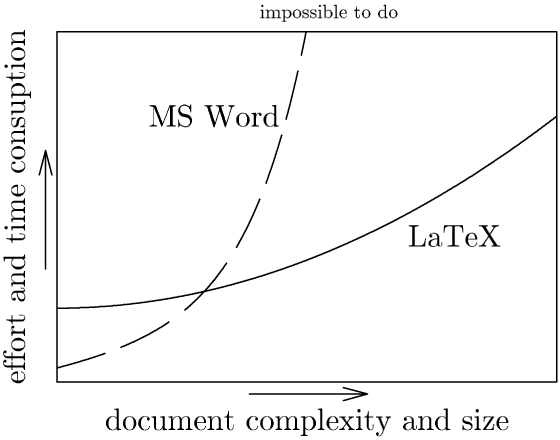
\includegraphics[width=190px]{img/when_use_latex.png}
        \caption{Kdy se vyplatí použít \LaTeX}
	\end{figure}
	    \srctext{Zdroj obrázku: \url{http://www.pinteric.com/miktex.html}}
\end{frame}

\begin{frame}
    \frametitle{Jak na to}
	Co potřebuji pro zprovoznění \LaTeX{\lower .5ex\hbox {U}}:
    \begin{center}
		\begin{enumerate} %[<+->]
			\item Překládací software
				\begin{itemize}
					\item \href{https://tug.org/texlive/}{TeX Live} [Windows, MacOsX, Linux]
					\item \href{https://miktex.org/}{MiKTex} [Windows]		
				\end{itemize}	
			\item Editor zdrojové kódu
				\begin{itemize}
					\item \href{http://www.xm1math.net/texmaker/}{Texmaker} [free - Windows, MacOsX, Linux]
					\item \href{https://atom.io/}{Atoms} [free - Windows, MacOsX, Linux]
					\item \href{http://www.pspad.com/cz/}{PSPad} [free - Windows]
					\item \href{https://notepad-plus-plus.org/}{Notepad++} [free - Windows]
				\end{itemize}			
		\end{enumerate}
    \end{center}
\end{frame}

\begin{frame}[fragile]
    \frametitle{Jak na to}
	Instalace Linux:
	\pause
	\vspace{5mm}
	\begin{lstlisting}[language=bash]
cfdisk /dev/hda && mkfs.xfs /dev/hda1 && mount /dev/hda1 /mnt/gentoo/ && chroot /mnt/gentoo/ && env-update && . /etc/profile && emerge sync && cd /usr/portage && scripts/bootsrap.sh && emerge system && emerge vim && vi /etc/fstab && emerge gentoo-dev-sources && cd /usr/src/linux && make menuconfig && make install modules_install && emerge gnome mozilla-firefox openoffice && emerge grub && cp /boot/grub/grub.conf.sample /boot/grub/grub.conf && vi /boot/grub/grub.conf && grub && init 6
	\end{lstlisting}
\end{frame}


\begin{frame}[fragile]
    \frametitle{Jak na to}
	Instalace Linux:

	\vspace{10mm}
	\begin{lstlisting}[language=bash]
# Debian/Ubuntu/Xubuntu
apt-get install (*@\textcolor{blue}{texlive texlive-lang-czechslovak texmaker}@*)
	\end{lstlisting}

	\pause
	\begin{lstlisting}[language=bash]
# Fedora
yum install (*@\textcolor{blue}{texlive-scheme-full texmaker}@*)
	\end{lstlisting}
	\vspace{10mm}

	\pause
	Překládáme příkazy
	\verb|pdflatex JMENO_SOUBORU.tex|
	
\end{frame}


\begin{frame}[fragile]
    \frametitle{Jak na to}
	Ukázka jednoduchého dokumentu v \LaTeX{\lower .5ex\hbox {U}}:
	\begin{center}
	\begin{lstlisting}[language=bettertex]
\documentclass[12pt]{article}
\begin{document}
Hello world!
$a^2+b^2=c^2$ %math mode
\end{document}
	\end{lstlisting}
	\end{center}
	Pozor na češtinu!
	\verb|\usepackage[utf8]{inputenc}|
\end{frame}

\begin{frame}[fragile]
    \frametitle{Výhody \LaTeX{\lower .5ex\hbox {U}}}
    \begin{center}
		\begin{enumerate}
			\item Jednotné formátování v dokumentu
			\item Sazba stránek a kapitol
			\item Generování obsahu
			\item Seznamy obrázků, tabulek
			\item Citace
			\item Poznámky 
			\item Odkazy v textu
			\item Vkládání vzorců
			\item Číslování stran	
			\item Odrážky, číslované seznamy
			\item Sloupce
		\end{enumerate}
    \end{center}
\end{frame}

\begin{frame}[fragile]
    \frametitle{Výhody \LaTeX{\lower .5ex\hbox {U}}}
    \framesubtitle{1. Jednotné formátování v dokumentu}
    \begin{center}
		\begin{itemize}
			\item používá všude stejný font
			\item a již v základu jsou pěkné :-)
			\item nestaráte se o formátování nadpisů,\\
			odkazů, poznámek, citací
		\end{itemize}
    \end{center}
\end{frame}

\begin{frame}[fragile]
    \frametitle{Výhody \LaTeX{\lower .5ex\hbox {U}}}
    \framesubtitle{2. Sazba stránek a kapitol}

    Nová stránka:
    \begin{lstlisting}[language=bettertex]
  \newpage % zacne na nove strance
    \end{lstlisting}

    Kapitoly:\\
\begin{lstlisting}[language=bettertex]
  % popis/ukazka
  \titulek[ text do obsahu ]{ nadpis }
  \titulek*{ nadpis } necislovany nadpis
\end{lstlisting}

    \begin{lstlisting}[language=bettertex]
  % realne pouziti
  \section{Nadpis prvniq urovne}
  \subsection{Nadpis druhe urovne}
  \subsubsection{Nadpis treti urovne}
    \end{lstlisting}
\end{frame}

\begin{frame}[fragile]
    \frametitle{Výhody \LaTeX{\lower .5ex\hbox {U}}}
    \framesubtitle{3. Generování obsahu}

	Lze provést přidáním jednoho příkazu a následně se aktualizuje při každém přeložení. 

    \begin{lstlisting}[language=bettertex]
  \tableofcontents
    \end{lstlisting}	    

	\vfill
	\textit{Pozor, většinou je potřeba přeložit dokument dvakrát, pro zobrazení změn v obsahu. Nebo lze automatický volat překladač dvakrát.}
\end{frame}

\begin{frame}[fragile]
    \frametitle{Výhody \LaTeX{\lower .5ex\hbox {U}}}
    \framesubtitle{4. Seznamy obrázků, vzorců, tabulek}
	
	Platí to samé jako pro obsah. 

    \begin{lstlisting}[language=bettertex]
  \listoffigures %seznam obrazku
  \listoftables %seznam tabulek
    \end{lstlisting}

	\vfill
	\textit{Pozor, většinou je potřeba přeložit dokument dvakrát, pro zobrazení změn v obsahu. Lze také překladač volat vždy dvakrát (lze nastavit v Texmakeru) n.}
    	       
\end{frame}

\begin{frame}[fragile]
    \frametitle{Výhody \LaTeX{\lower .5ex\hbox {U}}}
    \framesubtitle{5. Citace}
	
	Odkaz na citaci
    \begin{lstlisting}[language=bettertex]
  \cite{jmeno_odkazu}
    \end{lstlisting}
		
	
	Vytvořit citaci
	\begin{enumerate}[a)]
		\item pomocí prostředí \textit{thebibliography} 
			
		\item nástrojem \hologo{BibTeX}
		
	\end{enumerate}

	\vfill
	Více informací naleznete v dokumentu: \\
	\textit{ITY6 - Vytváření prezentací}
\end{frame}		

\begin{frame}[fragile]
    \frametitle{Výhody \LaTeX{\lower .5ex\hbox {U}}}
    \framesubtitle{6. Poznámky}	

	Poznámky pod čarou
    \begin{lstlisting}[language=bettertex]
  \footnote{text poznamky}
    \end{lstlisting}

	\pause
	\vfill
	...a to je všechno.
\end{frame}

\begin{frame}[fragile]
    \frametitle{Výhody \LaTeX{\lower .5ex\hbox {U}}}
    \framesubtitle{7. Odkazy v textu}
	
	\vfill
    \begin{lstlisting}[language=bettertex]
  %identifikuje objekt
  \label{jmeno_odkazu}

  %odkaz na cislo objektu
  \ref{cislo_odkazu}

  %odkaz na cislo stranky s objektem
  \pageref{cislo_stranky}
    \end{lstlisting}
	\vfill
\end{frame}



\begin{frame}[fragile]
    \frametitle{Výhody \LaTeX{\lower .5ex\hbox {U}}}
    \framesubtitle{8. Vkládání vzorců (1)}

	\LaTeX{\lower .5ex\hbox {U}} je nejmocnější nástroj na práci se vzorci.	

    \begin{lstlisting}[language=bettertex]
  $a^2+b^2=c^2$ 
  % $ - pro vkladani do textu
	\end{lstlisting}

	\vfill
	\begin{center}
    $a^2+b^2=c^2$
	\end{center}
	\vfill

    \begin{lstlisting}[language=bettertex]
  \begin{equation*}
  \lim_{x \to \infty}\frac{\sin^2 x + 
  \cos^2 x}{4} = y \nonumber
  \end{equation*}
    \end{lstlisting}
	\vfill
\end{frame}


\begin{frame}[fragile]
    \frametitle{Výhody \LaTeX{\lower .5ex\hbox {U}}}
    \framesubtitle{8. Vkládání vzorců (2)}
	
	\begin{equation*}
	\lim_{x \to \infty}\frac{\sin^2 x + \cos^2 x}{4} = y \nonumber
	\end{equation*}	
	
	Číslované vzorce \verb|\begin{equation}|:\\
	\begin{equation*}
		\int_a^b f(x) \mathrm{d}x = 
		-\int_b^a f(x) \mathrm{d}x 
	\end{equation*}
\end{frame}

\begin{frame}[fragile]
    \frametitle{Výhody \LaTeX{\lower .5ex\hbox {U}}}
    \framesubtitle{9. Číslování stran \footnote{\url{https://en.wikibooks.org/wiki/LaTeX/Counters}}}

    Nastavení a zobrazení čítače stránek na \verb|x|: 
    \begin{lstlisting}[language=bettertex]
  \setcounter{page}{x}
	\end{lstlisting}
	
	Nastavení a zobrazení čítače stránek od jedné:
    \begin{lstlisting}[language=bettertex]
  \setcounter{page}{1}
	\end{lstlisting}

	Nastavení způsob sazby čísla stránky:
    \begin{lstlisting}[language=bettertex]
  \pagenumbering{styl}
	\end{lstlisting}

    Nastavení pozice na stránce:
    \begin{lstlisting}[language=bettertex]
  \pagestyle{styl}
	\end{lstlisting}

\end{frame}

\begin{frame}[fragile]
    \frametitle{Výhody \LaTeX{\lower .5ex\hbox {U}}}
    \framesubtitle{10. Odrážky, číslované seznamy (1)}
    
    \begin{multicols}{2}
    Odrážky
    \begin{lstlisting}[language=bettertex]
 \begin{itemize}
   \item prvni odrazka
   \item druha odrazka
 \end{itemize}
    \end{lstlisting}
    
    \begin{itemize}
		\item první odrážka
		\item druhá odrážka
	\end{itemize}
    
    Číslované seznamy
    \begin{lstlisting}[language=bettertex]
 \begin{enumerate}
   \item prvni polozka
   \item druha polozka
 \end{enumerate}
    \end{lstlisting}
		\begin{enumerate}
			\item první položka
			\item druhá položka
		\end{enumerate}

    \end{multicols}
\end{frame}

\begin{frame}[fragile]
    \frametitle{Výhody \LaTeX{\lower .5ex\hbox {U}}}
    \framesubtitle{10. Odrážky, číslované seznamy (2)}
        
    Číslované seznamy -- zanořování
	\vspace{3mm}
    \begin{lstlisting}[language=bettertex]
 \begin{enumerate}[a)]
   \item prvni polozka
     \begin{enumerate}
       \item prvni pod polozka
       \item druha pod polozka
     \end{enumerate}
   \item druha polozka
 \end{enumerate}
    \end{lstlisting}

\end{frame}

\begin{frame}[fragile]
    \frametitle{Výhody \LaTeX{\lower .5ex\hbox {U}}}
    \framesubtitle{10. Odrážky, číslované seznamy (3)}
    
    Číslované seznamy -- zanořování
		\begin{enumerate}
			\item první položka
			\begin{enumerate}
				\item první pod položka
				\item druhá pod položka
			\end{enumerate}			
			\item druhá položka
		\end{enumerate}
		
	Změna čísel na písmena: \verb|\begin{enumerate}[a)]|	
		\begin{enumerate}[a)]
			\item první položka
			\begin{enumerate}
				\item první pod položka
				\item druhá pod položka
			\end{enumerate}			
			\item druhá položka
		\end{enumerate}		

\end{frame}

\begin{frame}[fragile]
    \frametitle{Výhody \LaTeX{\lower .5ex\hbox {U}}}
    \framesubtitle{11. Sloupce}
	\begin{lstlisting}[language=bettertex]
  \begin{multicols}{2}
    Lorem ipsum dolor sit amet, consectetur
    adipiscing elit. Proin tincidunt mollis 
    nisl, in finibus dolor accumsan ultricies. 
    Integer consectetur purus eu lacus sodales.
  \end{multicols}
	\end{lstlisting}

		\begin{multicols}{2}
	Lorem ipsum dolor sit amet, consectetur adipiscing elit. Proin tincidunt mollis nisl, in finibus dolor accumsan ultricies. Integer consectetur purus eu lacus sodales consectetur. 
		\end{multicols}

	
\end{frame}

\begin{frame}[fragile]
    \frametitle{"Slabiny"}
    \framesubtitle{1. Obrázky}
    \begin{itemize}
    	\item složitější pozicování
    	\item \LaTeX{ }určí, kde obrázek bude
    	\item problémy s překryvem 
    \end{itemize}
	\begin{lstlisting}[language=bettertex]
  \begin{figure}[H]
    \includegraphics[width=220px]{img.png}
    \caption{Popisek k obrazku}
  \end{figure}
	\end{lstlisting}	
\end{frame}

\begin{frame}[fragile]
    \frametitle{"Slabiny"}
    \framesubtitle{2. Tabulky (1)}
	\begin{lstlisting}[language=bettertex]
\begin{table}
  \begin{tabular}{l | c | c | c | c }
    Competitor Name & Swim & Cycle & Run & Total \\
    \hline \hline
    John T   & 13:04 & 24:15 & 18:34 & 55:53 \\ 
    Norman P & 8:00  & 22:45 & 23:02 & 53:47 \\
    Alex K   & 14:00 & 28:00 & n/a   & n/a   \\
    Sarah H  & 9:22  & 21:10 & 24:03 & 54:35 
  \end{tabular}
  \caption{Triathlon results}
\end{table}    
	\end{lstlisting}	
\end{frame}

\begin{frame}[fragile]
    \frametitle{"Slabiny"}
    2. Tabulky (2)
    
	\begin{itemize}
		\item jednoduché tabulky lze dělat ručně
		\item složitější tvořte pomocnými nástroji \footnote{\url{http://www.tablesgenerator.com/}}
		\item ... nebo vlastními skripty
	\end{itemize}	    
    
\begin{table}
\begin{tabular}{l | c | c | c | c }
Competitor Name & Swim & Cycle & Run & Total \\
\hline \hline
John T          & 13:04 & 24:15 & 18:34 & 55:53 \\ 
Norman P        & 8:00  & 22:45 & 23:02 & 53:47\\
Alex K          & 14:00 & 28:00 & n/a   & n/a\\
Sarah H         & 9:22  & 21:10 & 24:03 & 54:35 
\end{tabular}
\caption{Triathlon results}
\end{table}    

\srctext{Zdroj tabulky: \url{https://cs.sharelatex.com/blog/2013/08/14/beamer-series-pt2.html}}

\end{frame}


\begin{frame}[fragile]
    \frametitle{Prezentace \LaTeX{\lower .5ex\hbox {U}}}
    Právě ji vidíte!
    
    Kdy použít:
    \begin{itemize}
    	\item chci sázet matematiku nebo zdrojový kód
    	\item složitější struktura prezentace
    	\item univerzitní prostředí
    \end{itemize}
    
    Kdy nepoužívat:
        \begin{itemize}
    	\item propagační materiály (\LaTeX{}nedělá moc COOL prezentace)
    	\item krátká prezentace s několika slajdy
    	\item velké množství obrázků
    \end{itemize}
\end{frame}

\begin{frame}[fragile]
    \frametitle{A co dál?} % \LaTeX{\lower .5ex\hbox {U}}
    
    
    Kdy použít:
    \begin{itemize}
    	\item \LaTeX{ }lze verzovat\footnote{\href{GitHub}{\url{https://github.com}}}
    	\item Vyzkoušejte Pandoc\footnote{\url{http://pandoc.org/}} (konvertor dokumentů)
    	\item \LaTeX{ }jde dobře kombinovat s programováním
		\begin{itemize}
	    	 \item Gnuplot\footnote{\url{http://gnuplot.sourceforge.net/}} - skriptové generování grafů
	    	 \item skript pro generování tabulek
	   	\end{itemize}		    	
    \end{itemize}

\end{frame}


\begin{frame}[fragile]
	\vfill
    \begin{center}
        {\huge </latex>}

		\vspace{10mm}
		Q \& A?
	\end{center}
	\vfill
\end{frame}


\end{document}

%---------------------------------------------------------------------

\begin{multicols}{2}
Lorem ipsum dolor sit amet, consectetur adipiscing elit. Proin tincidunt mollis nisl, in finibus dolor accumsan ultricies. Integer consectetur purus eu lacus sodales consectetur. Donec fermentum lacinia mi, ac malesuada nisi convallis in. Phasellus aliquam quam elit, hendrerit feugiat nunc pulvinar non.
\end{multicols}

\begin{frame}[fragile]
    \frametitle{Výhody \LaTeX{\lower .5ex\hbox {U}}}
    12. Matice

	\begin{array}{cccc}
    a^{11} \& a^{12} \& \hdots \& a^{1n} \\
    a^{21} \& a^{22} \& \hdots \& a^{2n} \\
    \vdots \& \vdots \& \ddots \& \vdots \\
    a^{m1} \& a^{m2} \& \hdots \& a^{mn} \\
	\end{array} 
\end{frame}
